% ===========================================================================
\chapter{Terminology}\jchap{専門用語}
% [o] LABEL
\label{chap:Terminology}
\label{sec:Terminology}
% [o] INDEX DESTINATIOn (DEF)
\ifor{Terminology}{専門用語}{せんもんようご}{Fachbegriffe}
% [o] INDEX TARGET

The following sections (ordered Latin alphabetically) can be used by itself to
understand some key concepts of Japanese language by explaining keywords
{専門用語} {【せんもんようご】}.

% A
% B
% C
% D
% ---------------------------------------------------------------------------
\section{Dakuten}\jsec{濁点} \label{sec:Dakuten}
\ithree{diacritic sign}{濁点}{Diakritisches Zeichen}
\ithree{diacritic sign}{だくてん}{Nigorierungszeichen}
\ithree{Umlaut}{ウムラウト}{Umlaut}
\ithree{syllable}{音節}{Silbe}

The \textbf{Dakuten} - Japanese {濁点} {【だくてん】} - is a diacritic sign.
Similar to the German Umlaut.  The {濁点} is referenced colloquial as {点々}
{【てんてん】}.  It us used to in {仮名} \hyperref[sec:Syllable]{syllabaries}
to mark a consonant to be pronounced voiced. Two strokes {「゙」} are used near
the Katakana letter.  For other {濁点}, please see \nameref{sec:Iteration} on
page \pageref{sec:Iteration}.

    % label sec:Dakuten
% ---------------------------------------------------------------------------
\section{Diphthong}\jsec{二重母音} \label{sec:Diphthong}
\ithree{diphthong}{二重母音}{Diphthong}
\ithree{diphthong}{にじゅうぼいん}{Diphthong}
\ithree{syllable}{音節}{Silbe}
\ija{「アエ」}
\ija{「アイ」}
\ija{「アウ」}
\ija{「アオ」}
\ija{「ウエ」}
\ija{「ウイ」}
\ija{「オエ」}
\ija{「オイ」}
\ija{「オウ」}

A \textbf{diphthong} {二重母音} {【にじゅうぼいん】} is a sound that is
constructed from two different sounds that glide into each other while
pronouncing and form a \hyperref[sec:Syllable]{syllable}. A \textbf{diphthong}
is made out of vocals.  Examples for a \textbf{diphthong} in Japanese are {姪}
|me.i| and {甥} |o.i|.  Also  {「アエ」}, {「アイ」}, {「アウ」},
{「アオ」}、{「ウエ」}, {「ウイ」}, {「オエ」}, {「オイ」} or {「オウ」} are
likely to appear as a \textbf{diphthong} in normal conversation in Japanese.
However, they becomes vowel connections when it is pronounced slowly and it is
treated as two vowels in the consciousness of the Japanese speaker.
  % label sec:Diphthong
% E
% F
% ---------------------------------------------------------------------------
\section{Furigana - 振り仮名} \label{sec:Furigana}


The Japanese \textbf{Furigana} - written in Japanese {振り仮名} {【ふりがな】}
- is an aid for reading \hyperref[sec:Kanji]{Kanji}. \textbf{Furigana} are
\hyperref[sec:Kana]{Kana}, so basically \hyperref[sec:Hiragana]{Hiragana} or
\hyperref[sec:Katakana]{Katakana}. \textbf{Furigana} are written next to the
character (mostly \hyperref[sec:Kanji]{Kanji}) which reading can not be
expected to be know mostly as annotative glosses. At first unknown or difficult
\hyperref[sec:Kanji]{Kanji} are candidates for \textbf{Furigana} but also in
books for Children some if not all \hyperref[sec:Kanji]{Kanji} have
\textbf{Furigana}. But even in books for learning English for example
\textbf{Furigana} can be found next to words written in
\hyperref[sec:Romaji]{Rōmaji}.

Text written horizontally \textbf{Furigana} are written mostly above the
referenced character. In vertically written text \textbf{Furigana} is written
on the right site next to the character. Good \textbf{Furigana} tries to place
the reading distinguishable to each character separately. So the
first example (Kanji+Hiragana) is not good. While the second (Kanji+Hiragana)
is a good usage of \textbf{Furigana}. 

\begin{center}
\begin{tabular}{rl}
 \normalsize over:&\Huge \ruby{東京}{とうきょう}
 \ruby{東}{とう}\ruby{京}{きょう}
 \ruby{東}{トー}\ruby{京}{キョー}
 \ruby{東}{tō}\ruby{京}{kyō} \\
 \normalsize behind:& \Huge 東京(とうきょう) 東京【とうきょう】\\
 \end{tabular}
\end{center}


Vertically written Tōkyō as it also can be seen on many signs.

\begin{center}
\setCJKfamilyfont{cjk-vert}[Script=CJK,RawFeature=vertical]{IPAPMincho}
\renewcommand{\rubysep}{-0.5ex}
%\raisebox{-.5\height}{
%\fbox{
\rotatebox{-90}{
\begin{minipage}{2.0cm} \CJKfamily{cjk-vert}
\Huge \ruby{東}{とう}\ruby{京}{ きょう}
\end{minipage}
%}
%}
}
\end{center}
\bigskip

Other names for \textbf{Furigana} are ruby/rubi or yomigana {読み仮名}
{【よみがな】}.  Ruby (Japanese {ルビ} /rubi/) is also a annotation system that
can be used in \LaTeX or HTML. Rubi are  also common in China, Taiwan and
Korea. 

A common example for using \textbf{Furigana} for adults:

\begin{center}
\Huge \ruby{地球}{ふるさと} 
\end{center}

In science fictions some astronaut could use the Japanese word {ふるさと}
/furusato/  with the meaning of "my hometown" to refer to the planet Earth ( =
{地球}{【ちきゅう】}). Or to make it more fancy and international (may be also
with connotation that Japan has no space in the future):

\begin{center}
\Huge \ruby{地球}{アース} 
\end{center}

Here {アース} refers to 'earth', but {地球} is better understandable by the
Japanese audience.

   % label sec:Furigana
% G
% H
% ---------------------------------------------------------------------------
\section{Handakuten - 半濁点} \label{sec:Handakuten}

In Japanese two different {濁点} {【だくてん】} are used. The {濁点}  and  the
{半濁点} {【はんだくてん】} has the marker of a little circle {「゚」} and is
therefore colloquially described as {丸} {【まる】} and indicates when the
pronunciation shifts from |h| to |p|.

 % label sec:Handakuten
% ---------------------------------------------------------------------------
\section{Hepburn System}\jsec{ヘボン式}
%[o] LABEL
\label{sec:Hepburn}
\label{sec:HepburnSystem}
\label{sec:OlderHepburnSystem}
\label{sec:NewerHepburnSystem}
% [o] INDEX
\ifor{Hepburn System}{ヘボン式}{へぼんしき}{Hepburn System}
\ifor{older Hepburn System}{標準ヘボン式ローマ字}{ひょうじゅん・へぼん・ろまあじ}{altes Hepburn System}
\ifor{newer Hepburn System}{修正ヘボン式ローマ字}{しゅうせい・へぼんしき・ろうまじ}{neueres Hepburn System}
\ithree{James Curtis Hepburn}{James Curtis Hepburn}{James Curtis Hepburn}

\begin{tabular}{lr}
\begin{minipage}{10.5cm}

The { ヘボン式} {【へぼんしき】} is one of the two most important transcription
systems for Japanese written \hyperref[sec:Mora]{morae} based language. The
{ヘボン式} is most used system worldwide and in Japan.

The word {ヘボン} (hebon) is an old writing of the name \textbf{Hepburn}, a US
American physician, translator, educator and lay Christian missionary, who used
it his first Japanese English Dictionary (3rd ed.) in 1867.

There are manly two different variants. The older {標準ヘボン式ローマ字}
{【ひょうじゅん・へぼん・ろまあじ】} variant, which is used for signs at train
stations. And the new variant the {修正ヘボン式ローマ字}
{【しゅうせい・へぼんしき・ろうまじ】} which is used as a revised system since
1954 in Kenkyusha dictionaries. Most western scientists are using this system.
This system is also used in this book.

\Link \href{http://en.wikipedia.org/wiki/James_Curtis_Hepburn}{Hepburn}

\end{minipage}
&
\raisebox{-.47\height}{
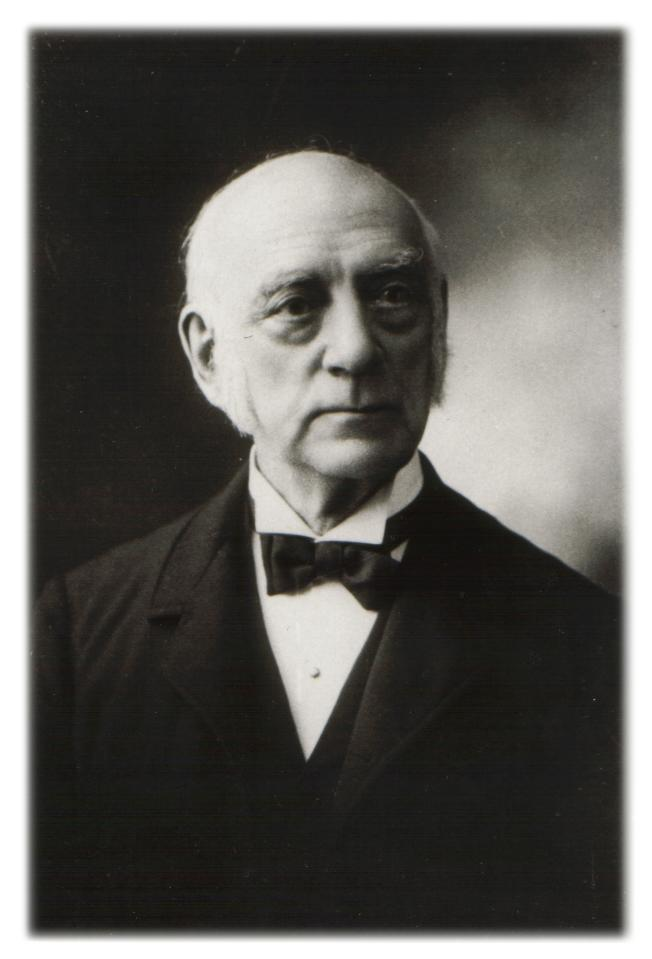
\includegraphics[scale=0.5,trim= 00 00 00 00]{../share/ei/James_Curtis_Hepburn.jpg}}
\\
\end{tabular}


    % label sec:Hepburn
% ---------------------------------------------------------------------------
\section{Hiragana - 平仮名} \label{sec:Hiragana}

TODO

{平仮名} {【ひらがな】}

   % label sec:Hiragana
% I
% ---------------------------------------------------------------------------
\section{Katakana Iteration Marks} \label{sec:Iteration}

As with {漢字} {【かんじ】} also {片仮名} has a iteration mark.  「ヽ」 and its
{濁点} {【だくてん】} form {「ヾ」}. This can only be
found in rare cases. For example the personal name Misuzu 【みすゞ】might
contain this character. And since the difference between the second last
and the last mora is only a change in pronunciation the {濁点} is added.

In vertical writing exist another iteration marker {くの字点} {【くのじてん】}
which consist out of two characters {「〳」+「〵」} and the {濁点} form
is {「〴」+「〵」}

  % label sec:Iteration
% J
% K
% ---------------------------------------------------------------------------
\section{Kana - 仮名} \label{sec:Kana}

TODO
       % label sec:Kana
% ---------------------------------------------------------------------------
\section{Kanji - 漢字} \label{sec:Kanji}

TODO
      % label sec:Kanji
% ---------------------------------------------------------------------------
\section{Katakana - 片仮名} \label{sec:Katakana}

At the same time as \hyperref[sec:Hiragana]{Hiragana}, also \textbf{Katakana}
letters where invented by simplifying the same Chinese characters used for
pronunciation.  However the look and feel of \textbf{Katakana} is more 'square'
not so 'rounded' as \hyperref[sec:Hiragana]{Hiragana}.

\textbf{Katakana} is used today for writing words of foreign origin and for
emphasizing (in commercials or \hyperref[sec:Manga]{Manga}) as well as word in
the fauna or flora.


   % label sec:Katakana
\section{Kunrei System}\jsec{訓令式ローマ字} 
% [o] LABEL
\label{sec:Kunrei}
\label{sec:KunreiSystem}
\label{sec:JapanSystemLatinLetters}
% [o] INDEX
\ifor{Kunrei system}{訓令式ローマ字}{くんれいろうまじ}{Kunrei System}
\ifor{Japan system Latin letters}{日本式ローマ字}{にほんしきろうまじ}{Lateinische Buchstaben des Japanischen Systems}
\ifor{Katakana}{片仮名}{かたかな}{Katakana}
\ifor{Gojūonzu}{五十音図}{ごじゅうおんず}{50 Laute Tafel}
\begin{tabular}{lr}
\begin{minipage}{9.6cm}

The modern \textbf{Kunrei} System {訓令式ローマ字} {【くんれいろうまじ】}  is
the official writing system of Japan. It was confirmed in 1994 by the Cabinet
and is available as ISO 3602:1989. The \textbf{Kunrei} System predecessor was
introduced 1985 by Dr. Aikitsu Tanakadatei ({田中舘愛橘}) as {日本式ローマ字}
{【にほんしきろうまじ】} (Nihon-/Nipponshikiromaji) and tries a more
systematical approach to map \hyperref[sec:Hiragana]{Hiragana} and
\hyperref[sec:Katakana]{Katakana} to equal Roman letters. The {五十音図}
{【ごじゅうおんず】} in the {訓令式ローマ字} is as follows:

\Link \href{http://en.wikipedia.org/wiki/Tanakadate_Aikitsu}{Tanakadate}

\end{minipage}
&
\raisebox{-.5\height}{
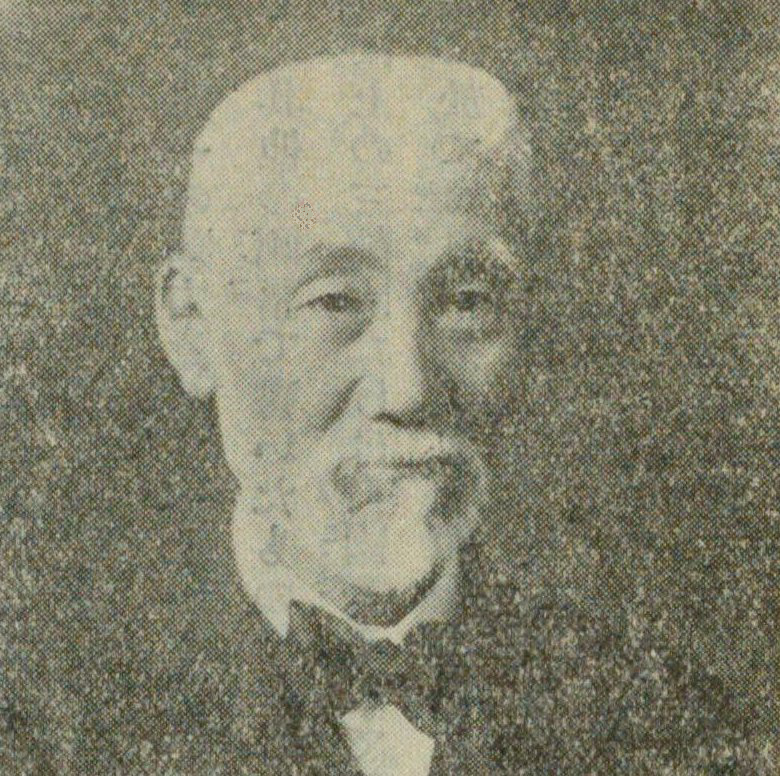
\includegraphics[scale=0.25,trim= 00 00 00 00]{../share/ei/Aikitsu_Tanakadate_r.jpg}}
\\
\end{tabular}


\Info{訓令式ローマ字 - Kunrei System}{
\begin{center}
\begin{tabular}{|c|c|c|c|c|}\hline
   a & i& u& e& o\\\hline
   ka&ki&ku&ke&ko\\\hline
   sa&si&su&se&so\\\hline
   ta&ti&tu&te&to\\\hline
   na&ni&nu&ne&no\\\hline
   ha&hi&hu&he&ho\\\hline
   ma&mi&mu&me&mo\\\hline
   ya&  &yu&  &yo\\\hline
   ra&ri&ru&re&ro\\\hline
   wa&  &  &  & o\\\hline
     &  &  &  & n\\\hline
\end{tabular}
\end{center}
}{true}

Even tough the system is official, many entities (like the train system) are
not using it. They use the Hepburn System.

The {訓令式ローマ字} is not part of this book. Please see \nameref{sec:Hepburn}
(on page \pageref{sec:Hepburn}) for the system in use.
     % label sec:Kunrei
% L
% M
% ---------------------------------------------------------------------------
\section{Manga - 漫画} \label{sec:Manga}

The Japanese version of comics is called \textbf{Manga} ({漫画} {【まんが】})
created on Japan or by Japanese authors. Some people say that \textbf{Manga} is
different from comics and deserve a name by its own. When \textbf{Manga} is
used in this book, then to distinguish it from comics in that sense that it is
written in Japanese posses a dynamic writing style\footnote{Conforming to a
style developed in Japan in the late 19th century.}  that is sometimes
challanging to its audience.

The term \textbf{Manga} for just Japanese comics is more used outside Japan. In
Japan all comics are referenced as \textbf{Manga} as well as with {コミック}
/komikku/ for all kinds of comics. The word \textbf{Manga} itself can be
translated as "whimsical drawings" or "impromptu sketches." and is used since
the late 18th century.


      % label sec:Manga
% ---------------------------------------------------------------------------
\section{Man'yōgana}\jsec{万葉仮名}
% [o] LABEL
\label{sec:Manyogana}
\label{sec:Manyoshu}
% [o] INDEX
\ifor{Man'yōgana}{万葉仮名}{まんようがな}{Man'yōgana}
\ifor{Man'yōshu}{万葉集}{まんようしゅう}{Man'yōshu}
\ifor{mora}{モーラ}{もーら}{Mora}
\ifor{Kanji}{漢字}{かんじ}{Kanji}
\ifor{Katakana}{片仮名}{かたかな}{Katakana}

The development of distinct Japanese writing begun 600 AD by writers and
scholars reducing some Chinese characters to its bare phonetic value. The
meaning of this characters where ignored. Around 760 a collection of Japanese
poetry was published, the \Link
\href{http://en.wikipedia.org/wiki/Man%27y%C5%8Dsh%C5%AB}{万葉集
【まんようしゅう】}, in which Chinese characters where uses as phonetic
letters. In regard to \textit{Man'yōshu} {万葉集} {【まんようしゅう】} the
characters are named {万葉仮名} {【まんようがな】}

The origin of the \textbf{Man'yōgana} script in poetry and art lead to some
problems in the understanding for the reader. Since the usage of phonetic
Chinese characters where mixed with regular Chinese characters and the
reasoning about which character to use was more form and shape aesthetic then
pragmatic, the meaning was difficult to grasp.

However the royal household or other scholars did not see a necessity to change
the status quo, because the high aim was to write poetry and other texts in
Chinese and \textbf{Man'yōgana} was considered appropriate only for notes,
diaries and love letters.

\Note{Note}{\footnotesize By the end of the 8th Century 970
\hyperref[sec:Kanji]{{漢字} {【かんじ】}} where used to pronounce the 90
\hyperref[sec:Mora]{morae}. This directly shows that there was no bijective map
between sound and character. For |ka| for example the following
\textbf{Man'yōgana} can be used {「可」}, {「何」}, {「加」}, {「架」},
{「香」}, {「蚊」}, {「迦」}. }

\newpage

The number of \textbf{Man'yōgana} from which \hyperref[sec:Katakana]{Katakana}
likely derived is smaller.  


\Hint{Man'yōgana used for creation of {片仮名} {【かたかな】}}{
\begin{center}
\begin{tabular}{|c||c|c|c|c|c|}\hline
 & a& i  & u  & e& o\\\hline\hline
-&阿&伊  &宇  &江&於\\\hline
k&加&機幾&久  &介&己\\\hline
s&散&之  &須  &世&曽\\\hline
t&多&千  &州川&天&止\\\hline
n&奈&仁  &奴  &祢&乃\\\hline
h&八&比  &不  &部&保\\\hline
m&末&三  &牟  &女&毛\\\hline
y&也&    &由  &  &與\\\hline
r&良&利  &流  &礼&呂\\\hline
w&和&井  &    &恵&乎\\\hline
*&尓&    &    &  &  \\\hline
\end{tabular}
\end{center}
}

The scientific term \textbf{Man'yōgana} is used by Western and Japanese
scientists. However it is not without critique. The term \textbf{Man'yōgana}
might lead to the illusion that it was a defined set of characters in use for
transcribing Chinese or writing Japanese texts or the second illusion that one
sound is represented by only  one \textbf{Man'yōgana}. Both is not true. First,
all Chinese Characters could in principle be used as \textbf{Man'yōgana} (and
therefore the term is basically useless). Actually the reason to chose one
character was sometimes just because out of aesthetic reasons, the shape or
some additional meaning. And second, normally many different
\textbf{Man'yōgana} (Chinese characters) where used for the same pronunciation
in the same text.  Making it efficient or easy was not the target of the
scholars using this kind of \hyperref[sec:PhoneticCharacter]{phonetic
characters} at that time.


\Link \href{http://en.wikipedia.org/wiki/Manyogana}{Man'yōgana}
\Link \href{http://en.wikipedia.org/wiki/Man%27y%C5%8Dsh%C5%AB}{万葉集}

  % label sec:Manyogana
% ---------------------------------------------------------------------------
\section{Mora - モーラ} \label{sec:Mora}

The concept of "mora"  (plural morae or moras; often symbolized μ) is used in
the science of linguistics. It describes a joint unit in pronunciation
(phonology) that constructs a syllable. The definition of a mora can vary.  In
Japanese the detection of morae is comparably simple. The world
{「チョコレート」} for example consist out of the following 5 morae
{「チョ」},{「コ」},{「レ」},{「ー」} and {「ト」} while it consist only out of
four \hyperref[sec:Syllable]{syllables} {(\hyperref[sec:Syllable]{音節}
【おんせつ】)}.

       % label sec:Mora
% N
% O
% ---------------------------------------------------------------------------
\section{Okurigana}\jsec{送り仮名}
% [o] LABEL
\label{sec:Okurigana}
\label{sec:Nokurigana}
% [o] INDEX
\ifor{Okurigana}{送り仮名}{おくりがな}{Okurigana}
\ifor{Katakana}{片仮名}{かたかな}{Katakana}
\ifor{Kana}{仮名}{かな}{Kana}
\ifor{Hiragana}{平仮名}{ひらがな}{Hiragana}
\ifor{Kanji}{漢字}{かんじ}{Kanji}
\ifor{Nokurigana}{ノくり仮名}{のくりがな}{Nokurigana}

The term \textbf{Okurigana} is written {送り仮名}{【おくりがな】} in Japanese,
but it is \textit{not} a script by its own as the name
\hyperref[sec:Kana]{Kana} suggest.  \textbf{Okurigana} are
\hyperref[sec:Kana]{Kana} but either \hyperref[sec:Hiragana]{Hiragana} or
\hyperref[sec:Katakana]{Katakana} that are used to write the ending of words in
most cases verbs. More precise \textbf{Okuriagna} are suffixes of
\hyperref[sec:Kanji]{Kanji}. After 1945 only
\hyperref[sec:Hiragana]{Hiragana} are used to write \textbf{Okurigana} while
before \hyperref[sec:Katakana]{Katakana} was used.

\textbf{Okurigana} are the mandatory compromise using static Chinese letters to
write the Japanese language. Next to make \hyperref[sec:Kanji]{Kanji} flexible
the other function is to mark the beginning are ending of words in sentences.

\textbf{Okurigana} have two purposes. (1) conjugate (a) verbs and (b)
adjectives. With very few exceptions\footnote{ {皮肉る} {【ひにくる】},
{牛耳る}  {【ぎゅうじる】} and {退治る} {【たいじる】}.}  Okuriagna will only
inflect \hyperref[sec:Kanji]{Kanji} as Kun'yomi.  (2) Change the meaning or
reading of a \hyperref[sec:Kanji]{Kanji} by different \textbf{Okurigana}.

\textit{Example: Okuriagana change the meaning (tense):}

\medskip
\begin{tabular}{ll}
\hspace{2cm}(1) {見る} {【みる】} & see \\
\hspace{2cm}(2) {見た} {【みた】} & saw \\
\end{tabular}

\medskip
In the above example the \textbf{Okurigana} of (1) is {「る」} and the
\textbf{Okurigana} of (2) is {「た」}.

\textit{Example: Okuriagana change the reading:}

\medskip
\begin{tabular}{ll}
\hspace{2cm}(1) {下さる} {【くださる】} & to give \\
\hspace{2cm}(2) {下りる} {【おりる】} &  to get off (a train for example)/ to descend \\
\hspace{2cm}(3) {下がる} {【さがる】} &  to dangle (intransitive)\\
\end{tabular}

\medskip
So in many cases the \textbf{Okurigana} directly after the
\hyperref[sec:Kanji]{Kanji} changes the meaning.

\textit{Example: Okuriagana change the meaning (transitivity) :}

\medskip
\begin{tabular}{ll}
\hspace{2cm}(1) {下がる} {【さがる】} &  to dangle (intransitive)\\
\hspace{2cm}(2){下げる} {【さげる】} &  to let off (transitive)\\
\end{tabular}

\medskip
As in the above case many Japanese verbs come in transitive and intransitive
pairs.  The reading of the \hyperref[sec:Kanji]{Kanji} is often shared.

\subsection*{Okurigana in the Middle}

\textbf{Okurigana} can also be found in the middle of Japanese words.

\textit{Example:}

\begin{center}\begin{tabular}{ll}
(1) {繰り返し} {【くりかえし】} &  to repeat\\
\end{tabular}\end{center}

\subsection*{Invisible Okuriagna - ノくり仮名}

The term {ノくり仮名} {【のくりがな】} was inspired by the site
\texttt{http://kanjidamage.com} but the writing was changed from Rōmaji to
Katakana+Okurigana+Kanji (The \hyperref[sec:Katakana]{Katakana} {「ノ」}
derives (of course) from the English 'no', and the word as such is a violation
of the Japanese \textbf{Okurigana}\footnote{Because
\hyperref[sec:Katakana]{Katakana} do not have \textbf{Okurigana}. But also in
case there would be no violation the /o/ of /okuri/ would be vilify to a
honorific prefix and then to be ripped out by the 'no' in a very non polite
way.} which describes a violation of \textbf{Okurigana}) Of course the term  is
not official, but quite funny in this case, that basically one should be very
angry with the fact that there are some Japanese words witch do have
\textbf{Okurigana} but are not written (but of course pronounced!).  The not so
funny part with those words is that if one knows the reading of the
\hyperref[sec:Kanji]{Kanji} it is impossible to look them up in a dictionary.
So lets strike back and spread the word of the ノくり仮名.

\begin{center}\begin{tabular}{ll}
(1) {取引} {取り引き} {【と(り)ひ(き)】} &  Transaction\\
(2) {受付} {受け付け} {【う(け)つ(け)】} &  Reception\\
\end{tabular}\end{center}


\Link \href{http://kanjidamage.com/tags/43}{http://kanjidamage.com/tags/43}








  % label sec:Okurigana
% P
\section{Phonetic Character - 表音文字} \label{sec:PhoneticCharacter}

In this document the term \textbf{Phonetic Character} ({表音文字}
{【ひょうおんもじ】}) refers genetically to a Chinese characters reading and
the usage of this character just for this purpose and \textit{not} for its
meaning. This common set expression has been used in avoidance of the term
\hyperref[sec:Manyogana]{Manyogana}. See the section \nameref{sec:Manyogana} on
page \pageref{sec:Manyogana} to understand the critique.

A \textbf{Phonetic Character} as to be distinguished from the linguistic term
\textit{phonogram} that describes a written character which represents a phonem
(speech sound) such as Latin alphabet or Japanese \hyperref[sec:Kana]{Kana}. 

 % label sec:PoneticCharacter
% Q
% R
% ---------------------------------------------------------------------------
\section{Radical}\jsec{部首}
% [o] LABEL
\label{sec:Radical}
% [o]  INDEX
\ifor{radical}{部首}{ぶしゅ}{Radikal}
\ifor{Kanji}{漢字}{かんじ}{Kanji}

A \textbf{radical} {部首} {【ぶしゅ】} is a root particle or character of a
Sino-Japanese character {漢字} {【かんじ】}. It is the most significant part of
a Sino-Japanese character. The concept was developed in China for Chinese
characters and is today known under the same name {部首} (pinyin: bùshǒu).

There is no general definition what a \textbf{radical} is or how many are
existing and it can vary a lot. The author of a dictionary has the power to
defined what a \textbf{radical} is and how much there will be in that
dictionary.

In more traditional Chinese or Japanese dictionaries a number of 214 or 244
\textbf{radicals} is quite common. However some modern approaches like the
\Link \href{http://www.hadamitzky.de/english/works_books.htm#KD}{\textit{The
Kanji Dictionary} of Marc Spahn and Wolfgang Hadamitzky from 1996} a totally
different number of 79 can be found.

\Note{Note}{\footnotesize Before buying a \hyperref[sec:Kanji]{Kanji}
dictionary, make sure that the \textbf{radical} system used suits your taste.
Sometimes it can be observed that Japanese dictionaries are stricter in the
definition of a \textbf{radical} because a given \hyperref[sec:Kanji]{Kanji}
can only be retrieved via exactly \textit{one} \textbf{radical}. While in many
Chinese dictionaries \textit{every} \textbf{radical} of a Chinese character can
be used to find it. The Japanese approach is of course good in terms of
systematic and didactic for learners, however it can take significant longer to
look up a character by \textbf{radical}.  }

    % label sec:Radical
% ---------------------------------------------------------------------------
\section{Rōmaji  - ローマ字} \label{sec:Romaji}


% ---------------------------------------------------------------------------
\ifor{Rōmaji}{ローマ字}{ろーまじ}{Rōmaji}

In temporary Japan words written in western letters become more popular and
some parts of the written language is already westernized, like (Indian/
Arabic) numbers written in horizontal text almost per default. This western
Latin letters are called \textbf{Rōmaji} and are written in Japanese as
{ローマ字} {【ろおまじ】}, even though some of them are from different origin
like Indian numbers for example.



The western characters are mainly used for writing numbers in the horizontal
writing. Also for abbreviations capital and small letters are used. Sometimes
they are modified. For example the measurement of distance in the metric entity
"km" occupies to places in western scripts "k" + "m" while it only hold one
place in Japanese {「㎞」} or even one place in
\hyperref[sec:Katakana]{Katakana}  {「㌔」}. While the latter is ambiguous to
us, because colloquial kilogram is referenced as only "kilo".

\Note{One Space Rōmaji}{\begin{center}\small
\begin{tabular}{ll}
\textit{Western Multiple Space Letters}&\textit{One Space Rōmaji}\\
mg&㎎\\
mm&㎜\\
kg&㎏\\
cm&㎝\\
km&㎞\\
qm&㎡\\
qcc&㏄\\
\end{tabular}
\end{center}
}

There are other shapes of Rōmaji for numbers or letters:

%\fontspec{IPAPMincho}
\fontspec{IPAPGothic}

\begin{center}
\begin{tabular}{ll}
Roman       &ⅠⅡⅢⅣⅤⅥⅦⅧⅨⅩⅪⅫ...\\
Blac circle & ❶❷❸❹❺❻❼❽❾❿...\\
Withe circle &①②③④⑤⑥⑦⑧⑨⑩...\\
Withe double circle & ⓵⓶⓷⓸⓹⓺⓻⓼⓽⓾...\\
Letters             &ⓐⓑⓒ...\\
\end{tabular}
\end{center}
\newpage
\fontspec{FreeSans}

There are also a number of incidents in typography where multiple Katakana are
condensed into one space, where normally only one Katakana would exist. In some
case the direction of writing is even diagonal. This part of exception are not
part of this document and should be viewed under the peculiar aesthetic of
Japanese printing.

\Note{One Space Katakana}{\begin{center}\small
\begin{tabular}{ll}
\textit{Western Meaning}&\textit{One Space Katakana}\\
&㌃\\
calorie&㌍\\
kilo&㌔\\
gram&㌘\\
centi-&㌢\\
cent&㌣\\
\$&㌦\\
t&㌧\\
\%&㌫\\
ha&㌶\\
pages&㌻\\
milli-&㍉\\
mbar (millibar)&㍊\\
m (meter)&㍍\\
l (liter)&㍑\\
&㍗\\
\end{tabular}
\end{center}
}

Citation of foreign books are also done in western letters an can pop up
without warning the middle of the text.
     % label sec:Romaji
% S
\section{Space Character}\jsec{空白文字} 
% [o] LABEL
\label{sec:SpaceCharacter}
% [o] INDEX DESTINATION (DEF)
\ifor{space character}{空白文字}{くうはく ・ もじ}{Leerzeichen}
% [o] INDEX TARGET
\ifor{Katakana}{片仮名}{かたかな}{Katakana}
\ifor{Kanji}{漢字}{かんじ}{Kanji}
\ifor{Hiragana}{平仮名}{ひらがな}{Hiragana}
\ifor{Rōmaji}{ローマ字}{ろーまじ}{Rōmaji}

The \textit{space character} in Western (Latin letter based) languages is used
to separate words. In antique texts a separation of words was \textbf{not}
common and those where difficult to read.  In the 7th century AD the word
separation was introduced. In the beginning of printed books the space wide was
fixed and to archive this the width of the letters where not fixed which
produced an easy to read text body.

The invention of typewriters and computers destroyed this approach of
aesthetically advanced typography. The typewriters had still a fixed (too
large) space width but also fixed letters. While the computer on screen behave
not better as a typewriter in the beginning and in printing, the spaces are
variable and the letters are fixed, the opposite of the elegant book printing
of the 15th century AD.

With the invention of Unicode the \textit{space character} is not longer a
singularity.  The Unicode fonts have now many\footnote{To give an example:
U+2008 Punctuation Space, U+2009 Thin Space, ..., U+FEFF Zero Width No-Break
Space, to just name a few.} \textit{space characters}. 

The Japanese computer fonts do have a \textit{space character}. Traditionally
more then one.  The most important \textit{space character} is the double wide
\textit{space character} which is exactly as wide as a
\hyperref[sec:Kanji]{Kanji} character. And the single wide space character that
is as wide as \hyperref[sec:Romaji]{Rōmaji} or half wide
\hyperref[sec:Hiragana]{Hiragana} or \hyperref[sec:Katakana]{Katakana}. 

However even though there is a \textit{space character} nowadays in Japanese
fonts it is \textbf{not} used to separate words from each other. Because of
this the word border can only be detected by heuristics and changes in scripts,
for example: \hyperref[sec:Katakana]{Katakana} to \hyperref[sec:Kanji]{Kanji},
\hyperref[sec:Hiragana]{Hiragana} to \hyperref[sec:Kanji]{Kanji},
\hyperref[sec:Katakana]{Katakana} to \hyperref[sec:Hiragana]{Hiragana} and so
on. Detecting words is a major task in learning Japanese.

The \textit{space character} in Japan is used to indent text to mark
paragraphs. To separate functional entities in the text like author from
heading. 

As a matter of fact the \textit{space character} in modern Japanese plays a
very unimportant role. 

This was not always so. In old Japanese there where an additional usage of
\textit{space characters} as {闕字} {【けつじ】} to leave space in front of
names of important persons or verbs to honor them.

\smallskip
\textbf{Example:}

\begin{center}\Padding\begin{tabular}{p{4cm}p{3cm}p{4cm}}
 {「  上様」} & {【うえさま】}      & Mister Ue \\
 {「登  城」} &  {【とう じょう】} & registered castle\\
\end{tabular}\end{center}
\smallskip

However this usage was abandoned in the Meiji era. 

\Link \href{http://ja.wikipedia.org/wiki/%E9%97%95%E5%AD%97}{http://ja.wikipedia.org/wiki/闕字}

 % sec:SpaceCharacter
% ---------------------------------------------------------------------------
\section{Syllable - 音節} \label{sec:Syllable}

A \textbf{syllable} {音節}  {【おんせつ】}  is a phonetic building block for
words. It influences the rhythm of a spoken language. In Western languages a
\textbf{syllable} is made out of one or more letters. In Japanese it is often
one character (of \hyperref[sec:Kana]{Kana}), but not always. For a better
understanding of the Japanese it is important to understand the concept of
\hyperref[sec:Mora]{mora}.

\Link \href{http://en.wikipedia.org/wiki/Syllable}{Syllable}
\Link \href{http://ja.wikipedia.org/wiki/%E9%9F%B3%E7%AF%80}{音節}

   % label sec:Syllable
% T
% U
% V
% W
% X
% Y
% Z

